\section{Experimentellt genomförande}
\label{sec:exper}
För att kunna analysera reaktionshastigheten behöver ni kunna följa
reaktionens gång som funktion av tid. Till ert förfogande kommer ni ha en
s.k. ``stopped-flow''-utrustning. Den fungerar enligt följande:

\begin{figure}[center]
  \centering
  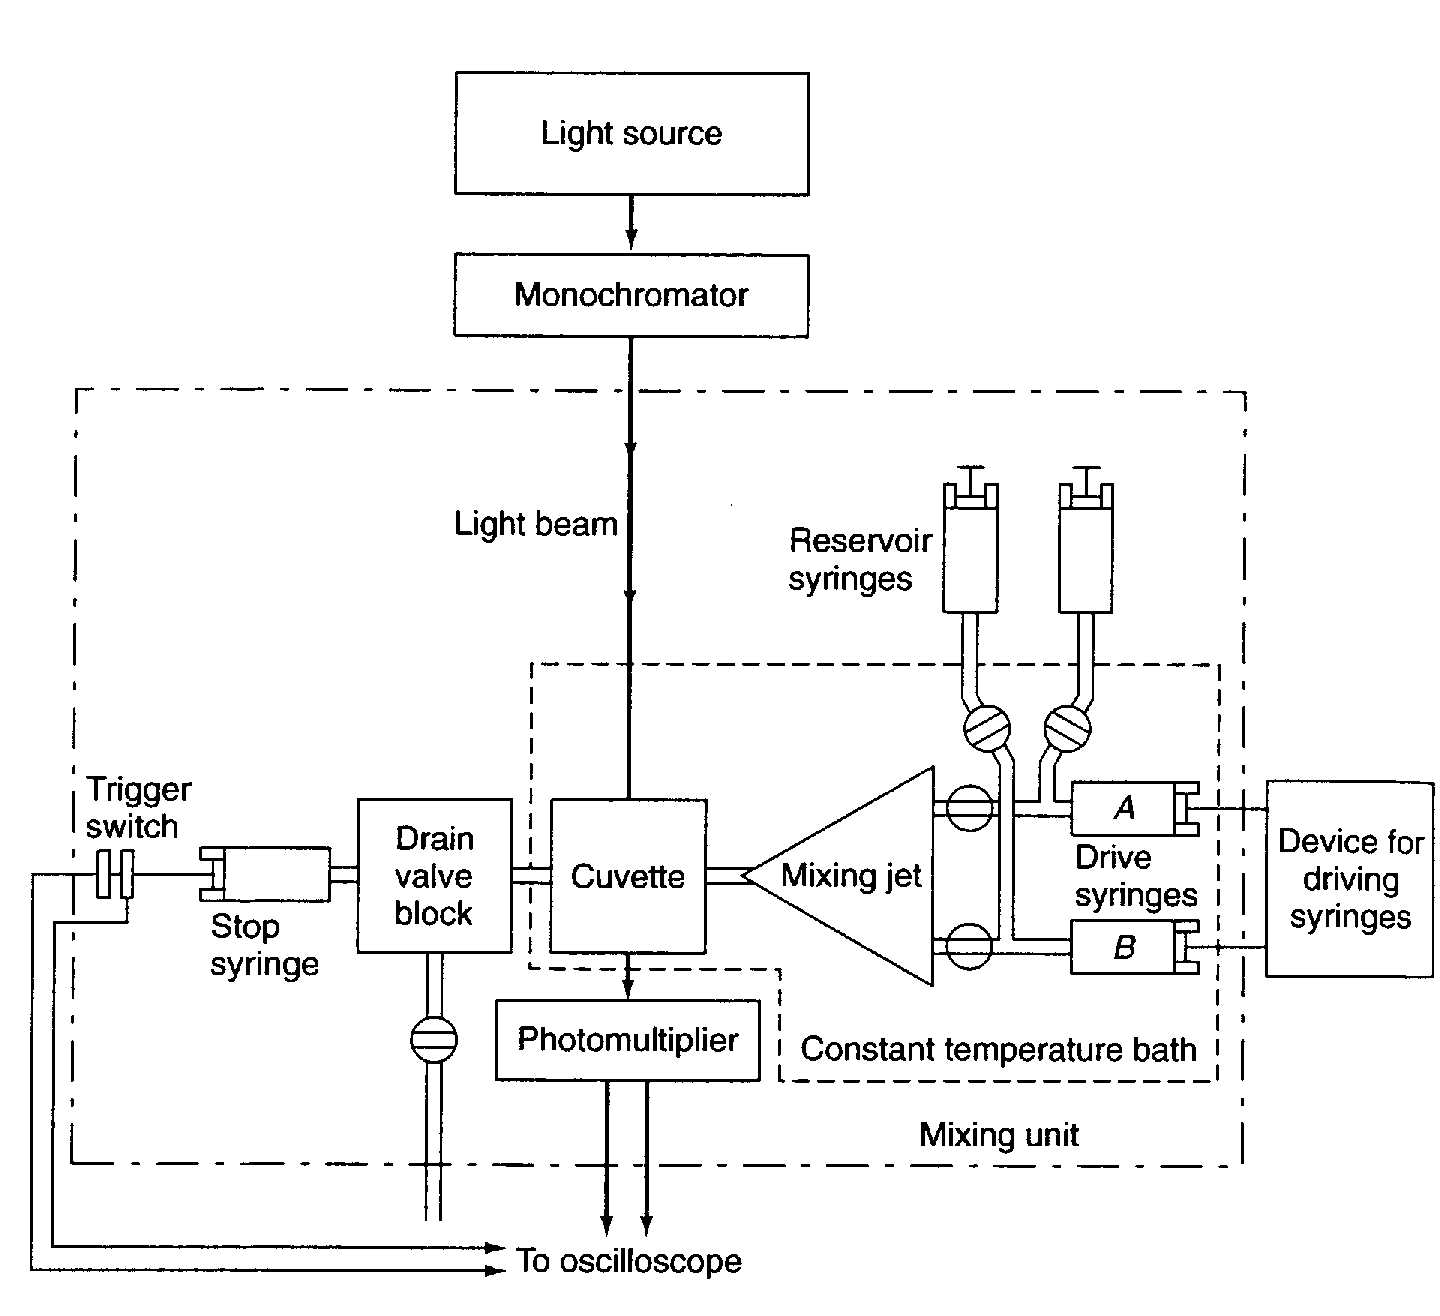
\includegraphics[scale=0.2]{fig/stopped_flow.png}
  \caption{Schematisk representation av stopped-flow utrustning}
  \label{fig:stopped-flow}
\end{figure}

Blandkammaren är termostaterad med hjälp av vattenbad som ni själva får
välja temperatur för. Ni kan börja era försök vid
rumstemperatur. Kyvettens längd är \SI{1}{\centi\metre} (vilket
tillsammans med extinktionskoefficienten  är något ni har nytta av att
veta när ni väljer koncentrations intervall för er reaktantlösning).

Istället för ett oscilloskåp kommer ni ha en dator med ett interface
skrivet i LabView. Handhavandet av programmet är beskrivet i
\cref{sec:labview}. Från varje försök kommer ni att erhålla dataserier med
absorbans som funktion av tid vid en våglängd som ni själva väljer.

\subsection{Stamlösningar}
För att bereda era reaktantlösningar kommer ni ha tillgång till följande
förberedda stamlösningar:

\begin{itemize}
\item \SI{1}{\Molar} \ce{NaClO4}
\item \SI{1}{\Molar} \ce{HClO4}
\item \SI{100}{\milli\Molar} \ce{KSCN}
\item \SI{100}{\milli\Molar} \ce{Fe(NO3)3}
\end{itemize}

\subsection{LabView interface}
\label{sec:labview}
\subsubsection{Förberedelser}
\begin{itemize}
\item Tänd lampan minst 5 minuter innan mätningarna.
\item Kontrollera att vattennivån i termostaten är tillräckligt hög.
Starta termostat och termometer.
\item Kolla att kylvattnet är på med hjälp av den röda flödesmätaren .
\item Sätt på kranvattnet.
\item Ställ in och invänta rätt temperatur, börja med den lägsta.
OBS! Vid alla mätningar och kalibreringar ska ``Stop'' vara nedtryckt på ``Start/Stop
Acquisition ``. Om programmet stängs av måste kalibreringen (med dest. vatten) göras om,
tryck därför aldrig på ``Exit''. Undvik att Juftbubblor kommer in i kyvetten.
\end{itemize}
\subsubsection{Kalibrering}
\begin{itemize}
\item Ställ ``Integration lime'' till 2 ms.
\item Blockera strålgången med metallplåten. Tryck på ``Dark''. Ta bort metallplåten.
\item Injicera destillerat vatten. Tryck på ``Ref''.
\item Kontrollera att transmissionen och absorptionen ser ut som den bör.
\item Byt sprutor och injicera tillräckligt med reaktantlösning så att komplexet bildas i kyvetten.
\item Gå in i absorptionstOnstret och bestäm vid vilken våglängd mätningarna ska göras genom
att välja ``Peak'' i Integral/peak-menyn.
\end{itemize}
\subsubsection{Mätning}
\begin{itemize}
\item Gå in på fliken ``Time mode''.
\item Välj ``As fast as possible", ``Save to file'' och ``Use a trigger''.
\item Tryck på ``Start'' så att den gröna lampan lyser (triggern aktiveras).
\item Vinkla samtliga T-kranar nedåt.
\item Injicera snabbt in ny reaktantlösning. Håll kvar greppet i 4 sekunder.
\item Välj alltid ``Replace'' när frågerutan dyker upp.
\end{itemize}

%%% Local Variables:
%%% mode: latex
%%% TeX-master: "../main"
%%% End:
